\chapter{Adaptierbarkeit}
\label{ch:adaptierbarkeit}
Die in Kapitel~\ref{ch:neuronalesNetz} ab Seite~\pageref{ch:neuronalesNetz} aufgebaute und erstellte Architektur soll
zusammen mit dem in Kapitel~\ref{ch:client} ab Seite~\pageref{ch:client} implementierten Frontend durch weitere
Maschinen oder Module erweitert und verbessert werden.

Eine Untersuchung soll zeigen, ob sowohl die Architektur als auch das Frontend so modular entwickelt wurden, dass sie
problemlos um weitere Maschinen oder Module erweitert werden können. Eventuelle Probleme im System oder in der
Architektur sollen gelößt werden.

Auch soll so auf neue Versionen oder anpassungen der bereits implementierten Maschine reagieren werden können.

Für dieses Ziel werden im folgenden Kapitel alle notwendigen Schritte zum einbinden einer Schlauchbeutelmaschine
behandelt und erläutert. Anschließend werden diese Schritt für Schritt umgesetzt.

Die Abbildung~\ref{fig:schematische_architektur_5} auf Seite~\pageref{fig:schematische_architektur_5} zeigt eine
schematische Erweiterung des Systems. Dort ist sehr gut ersichtlich, dass der API Connect Service eine zentrale Rolle
in der Erweiterbarkeit einnimmt.

\begin{figure}[h]
    \centering
    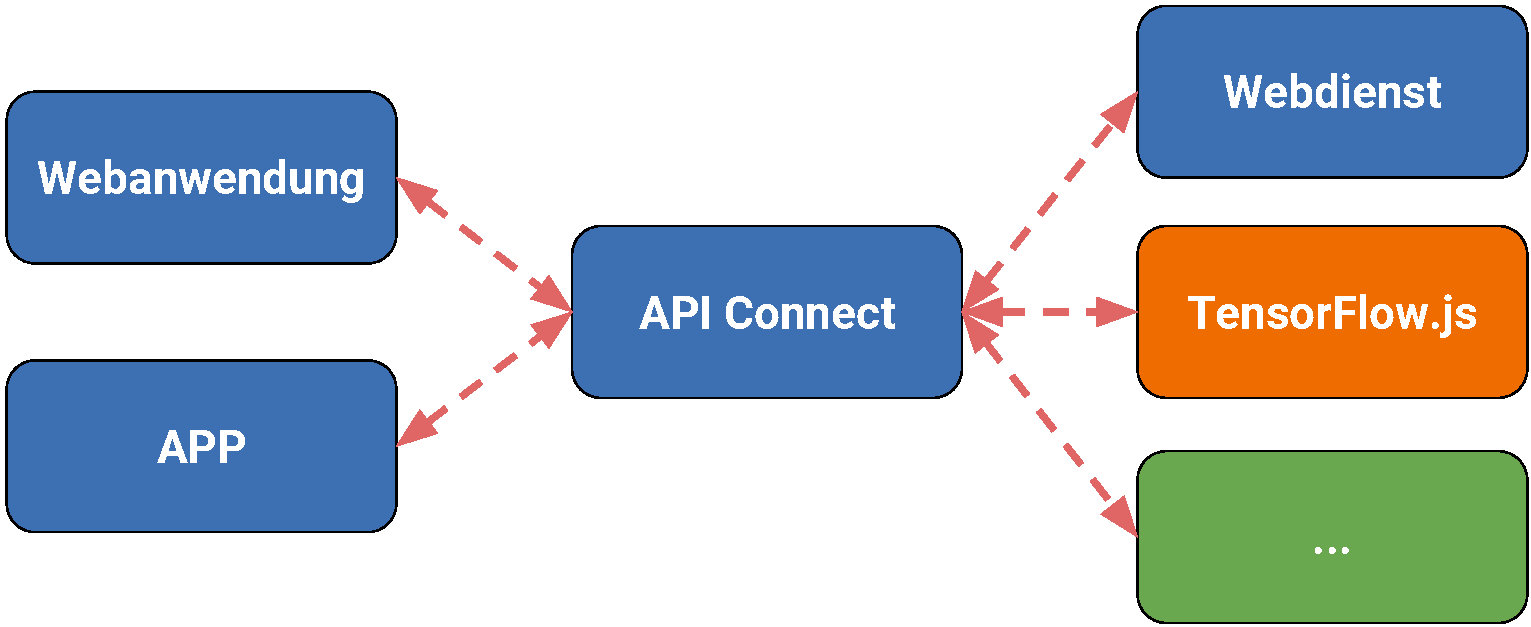
\includegraphics[width=\textwidth]{images/kapitel_5/architektur_schematisch.pdf}
    \caption{Schematische Darstellung der Adaptierbarkeit}
    \label{fig:schematische_architektur_5}
\end{figure}